\documentclass[a4paper,14pt]{article}

\usepackage{comment} % Para comentar várias linhas ao mesmo tempo

%matemática
\usepackage{amsmath}
\usepackage{amssymb}

%diagramação
\usepackage{extsizes}
\everymath{\displaystyle}
\usepackage{geometry}
\usepackage{fancyhdr}
\usepackage{multicol}
\usepackage{graphicx}
\usepackage[brazil]{babel}
\usepackage[shortlabels]{enumitem}
\usepackage{cancel}
\usepackage{textcomp}
\usepackage{tcolorbox}

%tabelas
\usepackage{array} % Para melhor formatação de tabelas
\usepackage{longtable}
\usepackage{booktabs}  % Para linhas horizontais mais bonitas
\usepackage{float}   % Para usar o modificador [H]
\usepackage{caption} % Para usar legendas em tabelas
\usepackage{wrapfig} % Para usar tabelas e figuras flutuantes
\usepackage{xcolor} % Para cores do fundo de tabelas
\usepackage{colortbl} % Para cores do fundo de tabelas

%tikzpicture
\begin{comment}
	\usepackage{tikz}
	\usepackage{scalerel}
	\usepackage{pict2e}
	\usepackage{tkz-euclide}
	\usetikzlibrary{calc}
	\usetikzlibrary{patterns,arrows.meta}
	\usetikzlibrary{shadows}
	\usetikzlibrary{external}
\end{comment}


%pgfplots
\usepackage{pgfplots}
\pgfplotsset{compat=newest}
\usepgfplotslibrary{statistics}
\usepgfplotslibrary{fillbetween}

%colours
\usepackage{xcolor}



\columnsep=2cm
\hoffset=0cm
\textwidth=8cm
\setlength{\columnseprule}{.1pt}
\setlength{\columnsep}{2cm}
\renewcommand{\headrulewidth}{0pt}
\geometry{top=1in, bottom=1in, left=0.7in, right=0.5in}

\pagestyle{fancy}
\fancyhf{}
\fancyfoot[C]{\thepage}

\begin{document}
	
	\noindent\textbf{6FMA113 - Matemática} 
	
	\begin{center}Ferramentas importantes em contagem (Versão estudante)
	\end{center}
	
	\noindent\textbf{Nome:} \underline{\hspace{10cm}}
	\noindent\textbf{Data:} \underline{\hspace{4cm}}
	
	%\section*{Questões de Matemática}
	
	\begin{multicols}{2}
		\noindent Para resolver problemas envolvendo contagem, podemos utilizar as seguintes ferramentas: \begin{itemize} 
		\item Listar todas as possibilidades.
		\item Utilizar tabelas.
		\item Utilizar diagramas de árvore.
		\item Utilizar diagramas de Venn.
		\end{itemize}
		\noindent\textsubscript{-----------------------------------------------------------------------}
		\begin{enumerate} 
			\item Pedro vai comprar um carro novo. O carro que ele escolheu tem a opção preto, prata, branco ou vermelho e o motor pode ser 1.4, 1.6 ou 2.0. Quantas opções distintas ele tem para o carro? \\
			Resolva listando todas as possibilidades. \\\\\\\\\\\\\\\\\\\\\\\\\\\\
			\item Bianca vai a um supermercado e deseja comprar um sorvete de massa. Ela pode escolher os sabores morango, chocolate ou limão e o tamanho dos potes são de 1,5 litro ou 2,0 litros. Quantas opções distintas ela tem para comprar um pote de sorvete de apenas 1 sabor? \\
			Resolva utilizando uma tabela. \newpage
			\item Em um jogo de $video game$ existem 6 ilhas. O início do jogo é na ilha 1 e o término é na ilha 6, porém os jogadores veteranos sabem que existe uma ilha secreta que faz a interligação entre as 6 ilhas, ou seja, é possível, por exemplo, passar da ilha 1 para a ilha 6 e finalizar o jogo sem ser necessário percorrer as outras ilhas. Ou também é possível passar da ilha 3 para a ilha 5 sem ser necessário percorrer a ilha 4. \\
			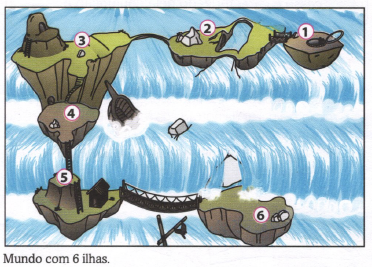
\includegraphics[width=1\linewidth]{6FMA113_imagens/imagem1}
			
			Sabendo que se pode passar pela ilha secreta apenas uma vez e que sempre se passa para alguma ilha à frente e nunca se volta, de quantas maneiras diferentes é possível terminar o jogo? \\\\\\\\\\\\\\\\\\\\\\\\
			\item Na escola de Gabriela só é permitido fazer um tipo de aula extracurricular: música, idiomas ou esportes. Na sala de Gabriela, 17 alunos praticam algum esporte, 11 estudam um novo idioma e 8 tocam algum instrumento. Quantos alunos dessa sala fazem a aula de música, ou idiomas, ou esportes? \\
			Resolva utilizando um diagrama de Venn. \newpage
			\item Cíntia e Emanuela disputarão 3 partidas de tênis de mesa, nas quais não há empates. Elas combinaram que se Cíntia vencer as 3 partidas, Cíntia será a grande vencedora. Já Emanuela precisa vencer a 1ª e a 3ª partidas e perder a 2ª partida para ser a grande vencedora. Em todos os casos, nenhuma das duas é a grande vencedora. Qual das amigas tem mais chances de ser a grande vencedora? \\
			Resolva pelo método que achar mais conveniente. \\\\\\\\\\\\\\\\\\\\\\\\\\\\\\\\\\\\\\\\\\\\\\\\\\\\\\
			\textbf{Desafio olímpico} \\\\
			(OBMEP) Os seis números 1, 2, 3, 4, 5 e 6 devem ser colocados nos quadrados de tal forma que eles fiquem em ordem crescente em cada linha (da esquerda para a direita) e em cada coluna (de cima para baixo). De quantas maneiras isso pode ser feito?
			\\ 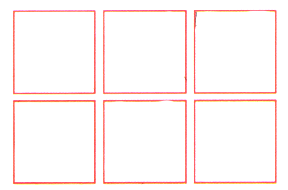
\includegraphics[width=1\linewidth]{6FMA113_imagens/imagem2} \\
			\begin{enumerate}[a)]
				\item 4
				\item 5
				\item 6
				\item 7
				\item 8 \newpage
			\end{enumerate}
			%9 a 12
			\item Em uma loja, os consumidores que fizessem uma compra participariam de um sorteio de brindes. Eles poderiam escolher chaveiros ou estojos, num total de 9 peças; ou canetas ou agendas, num total de 12 peças. De quantas formas os compradores poderiam fazer sua escolha? \\\\\\\\\\\\\\\\\\\\\\\\
			\item Suponha que no início de um jogo você tenha 80 pontos. A cada jogada, se vencer, você ganha 15 pontos; porém, se perder, perde 7 pontos. \\
			Ao final de três jogadas, quais serão as possíveis quantidades de pontos que você poderá ter? \\\\\\\\\\\\\\\\\\\\\\
			\item Em uma lanchonete, o cliente escolhe os ingredientes para montar seu hambúrger. \\
			As opções são queijo, alface, tomate, $bacon$, mostarda, $ketchup$ e maionese. Quantos hambúrgerers diferentes são possíveis de montar nessa lanchonete? \\\\\\\\\\\\\\\\\\\\\\\\\\\\
			\item De quantas formas um estudante pode "chutar" as respostas em uma prova de 12 questões tendo cada uma 4 alternativas?
		\end{enumerate}
		$~$ \\ $~$ \\ $~$ \\ $~$ \\ $~$ \\ $~$ \\ $~$ \\ $~$ \\ $~$ \\ $~$ \\ $~$ \\ $~$ \\ $~$ 
	\end{multicols}
\end{document}